\documentclass[a4paper]{article}

\def\nbook {Fluid Mechanics}
\def\nbookshort {FM}

% Shared preamble. The fallback lets the document build whether the working
% directory is its own folder or the project root.
\IfFileExists{headerfluidmechanics.tex}{\input{headerfluidmechanics}}{%%%%%%%%%%%%%%%%%%%%
% AUTHOR AND HEADER
% define \nbook
%%%%%%%%%%%%%%%%%%%%

\makeatletter
\ifx \nauthor\undefined
	\def\nauthor{David A. Lee}
\else
\fi

\author{\nbook \\ \small Pijush K. Kundu, Ira M. Cohen, and David R. Dowling \\ \small Solutions by \nauthor}
\date{}

%%%%%%%%%%%%%%%%%%%%
% PACKAGES
%%%%%%%%%%%%%%%%%%%%

\usepackage{alltt} 
\usepackage{amsfonts}
\usepackage{amsmath}
\usepackage{amssymb}
\usepackage{amsthm}
\usepackage{bm}
\usepackage{booktabs}
\usepackage{caption}
\usepackage{centernot}
\usepackage{enumitem}
\usepackage{fancyhdr}
\usepackage[T1]{fontenc}
\usepackage{graphicx}
\usepackage{lmodern}
\usepackage{mathdots}
\usepackage{mathtools}
\usepackage{microtype}
\usepackage{multirow}
\usepackage{pdflscape}
\usepackage{pgfplots}
\pgfplotsset{compat=1.18}
\usepackage{siunitx}
\usepackage{slashed}
\usepackage{tabularx}
\usepackage{tikz}
\usepackage{titletoc}
\usepackage{tkz-euclide}
\usepackage[normalem]{ulem}
\usepackage{url}
\usepackage[all]{xy}
\usepackage{imakeidx}

% fonts
% use \textsf to change to Computer Modern Bright
% \renewcommand{\sfdefault}{cmbr} % keeps default font Computer Modern Roman
\renewcommand{\familydefault}{\sfdefault} % set sans-serif as the default font

% makeindex for table of contents
\makeindex[intoc, title=Index]
\indexsetup{othercode={\lhead{ Index }}}

% table of contents remove numbering
\usepackage{tocloft} % for coloring subsections -- note that sections have standard document hyperlink coloring, i.e. color = doc
\setcounter{secnumdepth}{0} % remove numbering
\renewcommand{\cftsubsecfont}{\hypersetup{linkcolor=subsect!90}} % subsection coloring
\renewcommand{\contentsname}{\textsf{Table of Contents}}

% pagestyle
\pagestyle{fancyplain}

% header
\lhead{	\nouppercase{\leftmark} }
\ifx \nextra \undefined
  \rhead{
    \ifnum\thepage=1
    \else
      \nbookshort \  | \nauthor
    \fi}
\else
  \rhead{
    \ifnum\thepage=1
    \else
      \nbookshort (\nextra)
    \fi}
\fi

% proof environment

\newcommand{\prooffont}{\scshape}
\usepackage{xpatch}
\tracingpatches
\xpatchcmd{\proof}{\itshape}{\prooffont}{}{}

% Python environment (for typesetting Python code)

% Default fixed font does not support bold face
\DeclareFixedFont{\ttb}{T1}{txtt}{bx}{n}{8} % for bold
\DeclareFixedFont{\ttm}{T1}{txtt}{m}{n}{8}  % for normal

% Custom colors
\usepackage{color}
\definecolor{deepblue}{rgb}{0,0,0.5}
\definecolor{deepred}{rgb}{0.6,0,0}
\definecolor{deepgreen}{rgb}{0,0.5,0}

\usepackage{listings}

% Python style for highlighting
\newcommand\pythonstyle{\lstset{
language=Python,
basicstyle=\ttm,
morekeywords={self},              % Add keywords here
keywordstyle=\ttb\color{deepblue},
emph={MyClass,__init__},          % Custom highlighting
emphstyle=\ttb\color{deepred},    % Custom highlighting style
stringstyle=\color{deepgreen},
frame=tb,                         % Any extra options here
showstringspaces=false
}}


% Python environment
\lstnewenvironment{python}[1][]
{
\pythonstyle
\lstset{#1}
}
{}

% Python for external files
\newcommand\pythonexternal[2][]{{
\pythonstyle
\lstinputlisting[#1]{#2}}}

% Python for inline
\newcommand\pythoninline[1]{{\pythonstyle\lstinline!#1!}}

%%%%%%%%%%%%%
% FUNCTIONS %
%%%%%%%%%%%%%

\DeclarePairedDelimiter\abs{\lvert}{\rvert}%
% plain \abs{x} autosizes like \left| x \right|; \abs*{x} keeps fixed-size bars
\DeclarePairedDelimiter\absfixed{\lvert}{\rvert}%
\RenewDocumentCommand{\abs}{s}{\IfBooleanTF{#1}{\absfixed}{\absfixed*}}%
\DeclarePairedDelimiter\norm{\lVert}{\rVert}%

%%%%%%%%%%%%%%%%%%%%
% DOCUMENT GEOMETRY
%%%%%%%%%%%%%%%%%%%%

\ifx \ntrim \undefined
\else
  \usepackage{geometry}
  \geometry{
	  papersize={379pt, 699pt},
	  textwidth=345pt,
	  left=17pt,
	  top=54pt,
	  right=17pt,
  }
\fi

% maketitle statement
\title{}
\ifx \nisofficial \undefined
\let\@real@maketitle\maketitle
\renewcommand{\maketitle}{\@real@maketitle\begin{center}\begin{minipage}[c]{0.9\textwidth}\centering\footnotesize All errors, typographical and substantive, and other offenses, are entirely my own.\end{minipage}\end{center}}
\else
\fi

%%%%%%%%%%%%%%%%%%%%
% THEOREMS
%%%%%%%%%%%%%%%%%%%%

%\theoremstyle{definition}
\newtheorem*{axiom}{Axiom}
\newtheorem*{claim}{Claim}
\newtheorem*{conjecture}{Conjecture}
\newtheorem*{cor}{Corollary}
%\newtheorem*{dfn}{Definition}
\newtheorem*{eg}{Example}
\newtheorem*{ex}{Exercise}
%\newtheorem*{lemma}{Lemma}
\newtheorem*{prop}{Proposition}
%\newtheorem*{thm}{Theorem}
\newtheorem*{remark}{Remark}
\newtheorem*{warning}{Warning}

%%%%%%%%%%%%%%%%%%%%
% FORMATTING AESTHETICS
%%%%%%%%%%%%%%%%%%%%

% itemize bullets
\renewcommand{\labelitemi}{-}
\renewcommand{\labelitemii}{$\circ$}
\renewcommand{\labelenumi}{(\roman{*})}

% new page section
%\let\stdsection\section
%\renewcommand\section{\newpage\stdsection}

% new page subsection
%\let\stdsubsection\subsection
%\renewcommand\subsection{\newpage\stdsubsection}

%%%%%%%%%%%%%%%%%%%%
% \mathbb commands
%%%%%%%%%%%%%%%%%%%%

\newcommand{\C}{\mathbb{C}}
\newcommand{\N}{\mathbb{N}}
\newcommand{\Q}{\mathbb{Q}}
\newcommand{\R}{\mathbb{R}}
\newcommand{\Z}{\mathbb{Z}}

%%%%%%%%%%%%%%%%%%%%
% Complex Numbers
%%%%%%%%%%%%%%%%%%%%

\DeclareMathOperator{\Real}{Re}
\DeclareMathOperator{\Imag}{Im}

%%%%%%%%%%%%%%%%%%%%
% Probability Operators
%%%%%%%%%%%%%%%%%%%%

\DeclareMathOperator{\Bernoulli}{Bernoulli}
\DeclareMathOperator{\betaD}{Beta}
\DeclareMathOperator{\bias}{\textsf{bias}}
\DeclareMathOperator{\binomial}{Binomial}
\DeclareMathOperator{\corr}{Corr}
\DeclareMathOperator{\cov}{\textsf{Cov}}
\DeclareMathOperator{\Exp}{Exp}
\DeclareMathOperator{\gammaD}{Gamma}
\DeclareMathOperator{\mse}{\textsf{MSE}}
\DeclareMathOperator{\multinomial}{Multinomial}
\DeclareMathOperator{\Poisson}{Poisson}
\DeclareMathOperator{\sd}{sd}
\DeclareMathOperator{\se}{\textsf{se}}
\DeclareMathOperator{\Uniform}{Uniform}
\newcommand{\Prob}{\mathbb{P}}
\newcommand{\var}{\mathbb{V}}
\newcommand{\E}{\mathbb{E}}

%%%%%%%%%%%%%%%%%%%%
% TCOLORBOX CODE FROM SeniorMars
%%%%%%%%%%%%%%%%%%%%

%\usepackage[varbb]{newpxmath} changes math font to newpxmath
\usepackage{xfrac}
\usepackage[makeroom]{cancel}
\usepackage{mathtools}
\usepackage{bookmark}
\usepackage{enumitem}
\usepackage{hyperref,theoremref}
\hypersetup{
	pdftitle={Assignment},
	colorlinks=true, linkcolor=doc!90,
	bookmarksnumbered=true,
	bookmarksopen=true
}
\usepackage[most,many,breakable]{tcolorbox}
\usepackage{xcolor}
\usepackage{varwidth}
\usepackage{varwidth}
\usepackage{etoolbox}
%\usepackage{authblk}
\usepackage{nameref}
\usepackage{multicol,array}
\usepackage{tikz-cd}
\usepackage[ruled,vlined,linesnumbered]{algorithm2e}
\usepackage{comment} % enables the use of multi-line comments (\ifx \fi)
\usepackage{import}
\usepackage{xifthen}
\usepackage{pdfpages}
\usepackage{transparent}

\newcommand\mycommfont[1]{\footnotesize\ttfamily\textcolor{blue}{#1}}
\SetCommentSty{mycommfont}
\newcommand{\incfig}[1]{%
    \def\svgwidth{\columnwidth}
    \import{./figures/}{#1.pdf_tex}
}

\usepackage{tikzsymbols}
\usepackage{esint}
\usepackage{adjustbox}
\usetikzlibrary{calc}

% colors -- change them as you may!

\definecolor{myg}{RGB}{56, 140, 70}
\definecolor{myb}{RGB}{45, 111, 177}
\definecolor{myr}{RGB}{199, 68, 64}
\definecolor{mytheorembg}{HTML}{F2F2F9}
\definecolor{mytheoremfr}{HTML}{00007B}
\definecolor{mylenmabg}{HTML}{FFFAF8}
\definecolor{mylenmafr}{HTML}{983b0f}
\definecolor{mypropbg}{HTML}{f2fbfc}
\definecolor{mypropfr}{HTML}{191971}
\definecolor{myexamplebg}{HTML}{F2FBF8}
\definecolor{myexamplefr}{HTML}{88D6D1}
\definecolor{myexampleti}{HTML}{2A7F7F}
\definecolor{mydefinitbg}{HTML}{E5E5FF}
\definecolor{mydefinitfr}{HTML}{3F3FA3}
\definecolor{notesgreen}{RGB}{0,162,0}
\definecolor{myp}{RGB}{197, 92, 212}
\definecolor{mygr}{HTML}{880808}
\definecolor{myred}{RGB}{127,0,0}
\definecolor{myyellow}{RGB}{169,121,69}
\definecolor{myexercisebg}{HTML}{F2FBF8}
\definecolor{myexercisefg}{HTML}{88D6D1}
\definecolor{doc}{RGB}{0,0,255}
\definecolor{subsect}{RGB}{255,0,0}
\definecolor{question}{HTML}{4EB8DE}

%================================
% THEOREM BOX
%================================

%\providecommand\theoremnumber{}
\tcbuselibrary{theorems,skins,hooks}
\newtcbtheorem{Theorem}{Theorem}
{%
	enhanced,
	breakable,
	colback = mytheorembg,
	frame hidden,
	boxrule = 0sp,
	borderline west = {2pt}{0pt}{mytheoremfr},
	sharp corners,
	detach title,
	before upper = \tcbtitle\par\smallskip,
	coltitle = mytheoremfr,
	fonttitle = \bfseries\sffamily,
	description font = \mdseries,
	separator sign none,
	segmentation style={solid, mytheoremfr},
}
{th}


%================================
% Question BOX
%================================

\makeatletter
\newtcbtheorem{question}{Question}{enhanced,
	breakable,
	colback=white,
	colframe=question,
	attach boxed title to top left={yshift*=-\tcboxedtitleheight},
	fonttitle=\bfseries\sffamily,
	title={#2},
	boxed title size=title,
	boxed title style={%
			sharp corners,
			rounded corners=northwest,
			colback=tcbcolframe,
			boxrule=0pt,
		},
	underlay boxed title={%
			\path[fill=tcbcolframe] (title.south west)--(title.south east)
			to[out=0, in=180] ([xshift=5mm]title.east)--
			(title.center-|frame.east)
			[rounded corners=\kvtcb@arc] |-
			(frame.north) -| cycle;
		},
	#1
}{def}
\makeatother

%================================
% PROPERTIES BOX
%================================

\tcbuselibrary{theorems,skins,hooks}
\newtcbtheorem{Property}{Property}
{%
	enhanced,
	breakable,
	colback = mytheorembg,
	frame hidden,
	boxrule = 0sp,
	borderline west = {2pt}{0pt}{mytheoremfr},
	sharp corners,
	detach title,
	before upper = \tcbtitle\par\smallskip,
	coltitle = mytheoremfr,
	fonttitle = \bfseries\sffamily,
	description font = \mdseries,
	separator sign none,
	segmentation style={solid, mytheoremfr},
}
{th}

%================================
% LEMMA
%================================

\tcbuselibrary{theorems,skins,hooks}
\newtcbtheorem[number within=section]{Lemma}{Lemma}
{%
	enhanced,
	breakable,
	colback = mylenmabg,
	frame hidden,
	boxrule = 0sp,
	borderline west = {2pt}{0pt}{mylenmafr},
	sharp corners,
	detach title,
	before upper = \tcbtitle\par\smallskip,
	coltitle = mylenmafr,
	fonttitle = \bfseries\sffamily,
	description font = \mdseries,
	separator sign none,
	segmentation style={solid, mylenmafr},
}
{th}


% Commands for special boxes
\newcommand{\thm}[2]{\begin{Theorem*}{#1}{}#2\end{Theorem*}}
\newcommand{\qs}[2]{\begin{question*}{#1}{}#2\end{question*}}
\newcommand{\prp}[2]{\begin{Property*}{#1}{}#2\end{Property*}}
\newcommand{\lemma}[2]{\begin{Lemma*}{#1}{}#2\end{Lemma*}}
}

\begin{document}
\maketitle

\newpage
\tableofcontents

\newpage
\section{3 - Kinematics}

% QUESTION 1
\qs{3.1}{The gradient operator in Cartesian coordinates \( \!\left( x,y,z \right) \) is: \( \nabla = \pmb{e}_{x}\!\left( \partial / \partial x \right) + \pmb{e}_{y}\!\left( \partial / \partial y \right) + \pmb{e}_{z}\!\left( \partial / \partial z \right) \) where \( \pmb{e}_{x} \), \( \pmb{e}_{y} \), and \( \pmb{e}_{z} \) are the unit vectors. In cylindrical polar coordinates \( \!\left( R,\phi,z \right) \) having the same origin, (see Figure 3.3c), coordinates and unit vectors are related by: \( R = \sqrt{x^{2} + y^{2}} \), \( \phi = \tan^{-1}\!\left(y/x\right) \), and \( z = z \); and \( \pmb{e}_{R} = \pmb{e}_{x}\cos\!\left(\phi\right) + \pmb{e}_{y}\sin\!\left(\phi\right) \), \( \pmb{e}_{\phi} = -\pmb{e}_{x}\sin\!\left(\phi\right) + \pmb{e}_{y}\cos\!\left(\phi\right) \), and \( \pmb{e}_{z} = \pmb{e}_{z} \). Determine the following in the cylindrical polar coordinate system. [This exercise requires some mathematical patience.]
\begin{enumerate}[label=(\alph*)]
	\setcounter{enumi}{2}
	\item the divergence of the velocity field \( \nabla \cdot \pmb{u} \)
	\setcounter{enumi}{4}
	\item the advective acceleration term \( \!\left( \pmb{u} \cdot \nabla \right)\pmb{u} \)
\end{enumerate}}

\begin{enumerate}[label=(\alph*)]
	\setcounter{enumi}{2}
	\item First, the definitions for \( R \) and \( \phi \) collectively produce
	\[
		x = R \cos\!\left(\phi\right) \qquad y = R \sin\!\left(\phi\right) 
	\]
	Given the gradient operator in Cartesian coordinates, we will convert the Cartesian basis vectors and differential operators into their counterparts in cylindrical polar coordinates. We begin with the basis vector conversions. First we find the projections of \( \pmb{e}_{x} \) and \( \pmb{e}_{y} \) on \( \pmb{e}_{R} \) and \( \pmb{e}_{\phi} \); since \( \pmb{e}_{z} \) is unchanged we already know orthogonality exists.
	\begin{align*}
		\pmb{e}_{x} \cdot \pmb{e}_{R} & = \cos\!\left(\phi\right) \\
		\pmb{e}_{x} \cdot \pmb{e}_{\phi} & = -\sin\!\left(\phi\right) \\ 
		\pmb{e}_{y} \cdot \pmb{e}_{R} & = \sin\!\left(\phi\right) \\
		\pmb{e}_{y} \cdot \pmb{e}_{\phi} & = \cos\!\left(\phi\right)
	\end{align*}
	Expressing \( \pmb{e}_{x} \) and \( \pmb{e}_{y} \) in cylindrical polar coordinates:
	\begin{align*}
		\pmb{e}_{x} & = \cos\!\left(\phi\right)\pmb{e}_{R} - \sin\!\left(\phi\right)\pmb{e}_{\phi} \\
		\pmb{e}_{y} & = \sin\!\left(\phi\right)\pmb{e}_{R} + \cos\!\left(\phi\right)\pmb{e}_{\phi}
	\end{align*}
	which we also could have derived by identifying the corresponding linear combinations of the \( R \) and \( \phi \) basis vectors. 

	Following this, we convert the differential operators. Assisting in this endeavor is the total derivative:
	\begin{align*}
		\frac{\partial }{\partial x} & = \frac{\partial R}{\partial x}\frac{\partial }{\partial R} + \frac{\partial \phi}{\partial x}\frac{\partial }{\partial \phi} \\
		 & = \cos\!\left(\phi\right)\frac{\partial }{\partial R} - \frac{\sin\!\left(\phi\right)}{R}\frac{\partial }{\partial \phi} \\ 
		\frac{\partial }{\partial y} & = \frac{\partial R}{\partial y}\frac{\partial }{\partial R} + \frac{\partial \phi}{\partial y}\frac{\partial }{\partial \phi} \\
					     & = \sin\!\left(\phi\right)\frac{\partial }{\partial R} + \frac{\cos\!\left(\phi\right)}{R}\frac{\partial }{\partial \phi}
	\end{align*}
	where the partial derivatives can be derived from the definitions of \( R \) and \( \phi \). Substituting these pieces into the Cartesian gradient operator gives us
	\begin{alignat*}{2}
		& \!\left( \cos\!\left(\phi\right)\pmb{e}_{R} - \sin\!\left(\phi\right)\pmb{e}_{\theta} \right)\!\left( \cos\!\left(\phi\right)\frac{\partial }{\partial R} - \frac{\sin\!\left(\phi\right)}{R}\frac{\partial }{\partial \phi} \right) & \\
		& \quad + \!\left( \sin\!\left(\phi\right)\pmb{e}_{R} + \cos\!\left(\phi\right)\pmb{e}_{\theta} \right)\!\left( \sin\!\left(\phi\right)\frac{\partial }{\partial R} + \frac{\cos\!\left(\phi\right)}{R}\frac{\partial }{\partial \phi} \right) + \pmb{e}_{z}\frac{\partial }{\partial z} & \\
		& \qquad = \pmb{e}_{R}\frac{\partial }{\partial R} + \pmb{e}_{\phi}\frac{1}{R}\frac{\partial }{\partial \phi} + \pmb{e}_{z}\frac{\partial }{\partial z} &
	\end{alignat*}
	For \( \pmb{u} = \pmb{e}_{R}u_{R} + \pmb{e}_{\phi}u_{\phi} + \pmb{e}_{z}u_{z} \),
	\[
		\nabla \cdot \pmb{u} = \frac{\partial u_{R}}{\partial R} + \frac{1}{R}\frac{\partial u_{\phi}}{\partial \phi} + \frac{\partial u_{z}}{\partial z}
	\]
	\setcounter{enumi}{4}
	\item Compute
	\[
		\pmb{u} \cdot \nabla = u_{R}\frac{\partial }{\partial R} + \frac{u_{\phi}}{R}\frac{\partial }{\partial \phi} + u_{z}\frac{\partial }{\partial z} 
	\]
	For the next step, we will need to apply each component of \( \pmb{u} \) with our derived operator. Some facts to know that will assist with our computation are that
	\[
		 \frac{\partial \pmb{e}_{R}}{\partial \phi} = \pmb{e}_{\phi} \qquad \frac{\partial \pmb{e}_{\phi}}{\partial \phi} = -\pmb{e}_{R}
	\]
	are the only non-zero derivatives of any cylindrical polar basis vectors with respect to any variable. Each component is derived as
	\begin{align*}
		\!\left( \pmb{u} \cdot \nabla \right)\!\left( \pmb{e}_{R}u_{R} \right) & = \pmb{e}_{R}\!\left(  u_{R}\frac{\partial u_{R}}{\partial R} + \frac{u_{\phi}}{R}\frac{\partial u_{R}}{\partial \phi} + u_{z}\frac{\partial u_{R}}{\partial z} \right) + \pmb{e}_{\phi}\frac{u_{R}u_{\phi}}{R} \\
		\!\left( \pmb{u} \cdot \nabla \right)\!\left( \pmb{e}_{\phi}u_{\phi} \right) & = -\pmb{e}_{R}\frac{u^{2}_{\phi}}{R} + \pmb{e}_{\phi}\!\left( u_{R}\frac{\partial u_{\phi}}{\partial R} + \frac{u_{\phi}}{R}\frac{\partial u_{\phi}}{\partial \phi} + u_{z}\frac{\partial u_{\phi}}{\partial z} \right) \\ 
		\!\left( \pmb{u} \cdot \nabla \right)\!\left( \pmb{e}_{z}u_{z} \right) & = \pmb{e}_{z}\!\left(  u_{R}\frac{\partial u_{z}}{\partial R} + \frac{u_{\phi}}{R}\frac{\partial u_{z}}{\partial \phi} + u_{z}\frac{\partial u_{z}}{\partial z} \right)
	\end{align*}
	Summing, conclude
	\[
		\!\left( \pmb{u} \cdot \nabla \right)\pmb{u} = \pmb{e}_{R}\!\left[ \!\left( \pmb{u} \cdot \nabla \right)u_{R} - \frac{u^{2}_{\phi}}{R} \right] + \pmb{e}_{\phi}\!\left[ \!\left( \pmb{u} \cdot \nabla \right)u_{\phi} + \frac{u_{R}u_{\phi}}{R} \right] + \pmb{e}_{z}\!\left( \pmb{u} \cdot \nabla \right)u_{z} 
	\]
	Observe that the \( u^{2}_{\phi} / R \) is the centripetal acceleration term as it points inward towards the origin along the \( R \)-axis. The second of the unusual terms, \( u_{R}u_{\phi} / R \), can be thought of as the part of the radial velocity that is directed azimuthally as the fluid parcel moves. Conceptually, this is an angular momentum conservation term, which we will explore more in later chapters.
\end{enumerate}

\newpage
% QUESTION 2
\qs{3.2}{Consider Cartesian coordinates (as given in Exercise 3.1) and spherical polar coordinates \( \!\left( r,\theta,\phi \right) \) having the same origin (see Figure 3.3d). Here coordinates and unit vectors are related by: \( r = \sqrt{x^{2} + y^{2} + z^{2}} \), \( \theta = \tan^{-1}\!\left(\sqrt{x^{2} + y^{2}} / z\right) \), and \( \phi = \tan^{-1}\!\left(y/x\right) \); and \( \pmb{e}_{r} = \pmb{e}_{x}\cos\!\left(\phi\right)\sin\!\left(\theta\right) + \pmb{e}_{y}\sin\!\left(\phi\right)\sin\!\left(\theta\right) + \pmb{e}_{z}\cos\!\left(\theta\right) \), \(  \pmb{e}_{\theta} = \pmb{e}_{x}\cos\!\left(\phi\right)\cos\!\left(\theta\right) + \pmb{e}_{y}\sin\!\left(\phi\right)\cos\!\left(\theta\right) - \pmb{e}_{z}\sin\!\left(\theta\right) \), and \( \pmb{e}_{\phi} = -\pmb{e}_{x}\sin\!\left(\phi\right) + \pmb{e}_{y}\cos\!\left(\phi\right) \). In the spherical polar coordinate system, determine the following items. [This exercise requires mathematical patience.]
\begin{enumerate}[label=(\alph*)]
	\item \( \partial \pmb{e}_{r} / \partial \theta \), \( \partial \pmb{e}_{r} / \partial \phi \), \( \partial \pmb{e}_{\theta} / \partial \theta \), \( \partial \pmb{e}_{\theta} / \partial \phi \), and \( \partial \pmb{e}_{\phi} / \partial \phi \)
	\item the gradient operator \( \nabla \)
	\item the divergence of the velocity field \( \nabla \cdot \pmb{u} \)
	\item the Laplacian operator \( \nabla \cdot \nabla \equiv \nabla^{2} \)
	\item the advective acceleration term \( \!\left( \pmb{u} \cdot \nabla \right)\pmb{u} \)
\end{enumerate}}

\begin{enumerate}[label=(\alph*)]
	\item Compute
	\begin{align*}
		\frac{\partial \pmb{e}_{r}}{\partial \theta} & = \pmb{e}_{x}\cos\!\left(\phi\right)\cos\!\left(\theta\right) + \pmb{e}_{y}\sin\!\left(\phi\right)\cos\!\left(\theta\right) - \pmb{e}_{z}\sin\!\left(\theta\right) \\
		 & = \pmb{e}_{\theta} \\ 
		\frac{\partial \pmb{e}_{r}}{\partial \phi} & = -\pmb{e}_{x}\sin\!\left(\phi\right)\sin\!\left(\theta\right) + \pmb{e}_{y}\cos\!\left(\phi\right)\sin\!\left(\theta\right) \\
							   & = \pmb{e}_{\phi}\sin\!\left(\theta\right) \\
							\frac{\partial \pmb{e}_{\theta}}{\partial \theta} & = -\pmb{e}_{x}\cos\!\left(\phi\right)\sin\!\left(\theta\right) - \pmb{e}_{y}\sin\!\left(\phi\right)\sin\!\left(\theta\right) - \pmb{e}_{z}\cos\!\left(\theta\right) \\
													  & = -\pmb{e}_{r} \\
													\frac{\partial \pmb{e}_{\theta}}{\partial \phi} & = -\pmb{e}_{x}\sin\!\left(\phi\right)\cos\!\left(\theta\right) + \pmb{e}_{y}\cos\!\left(\phi\right)\cos\!\left(\theta\right) \\
																			& = \pmb{e}_{\phi}\cos\!\left(\theta\right) \\
																		\frac{\partial \pmb{e}_{\phi}}{\partial \phi} & = -\pmb{e}_{x}\cos\!\left(\phi\right) - \pmb{e}_{y}\sin\!\left(\phi\right) \\
																							      & = -\pmb{e}_{r}\sin\!\left(\theta\right) - \pmb{e}_{\theta}\cos\!\left(\theta\right)
	\end{align*}
	\item There is a brute force way and an elegant way. We will do it the painful way first so as to appreciate the elegance of a more geometric argument.

	First we write each Cartesian basis vector in terms of their spherical polar counterparts. A slick way to do this is to recognize that in matrix form
	\[
		\underbrace{\begin{bmatrix}
			\textcolor{blue}{\cos\!\left(\phi\right)\sin\!\left(\theta\right)} & \textcolor{red}{\sin\!\left(\phi\right)\sin\!\left(\theta\right)} & \textcolor{teal}{\cos\!\left(\theta\right)} \\
			\textcolor{blue}{\cos\!\left(\phi\right)\cos\!\left(\theta\right)} & \textcolor{red}{\sin\!\left(\phi\right)\cos\!\left(\theta\right)} & \textcolor{teal}{-\sin\!\left(\theta\right)} \\
			\textcolor{blue}{-\sin\!\left(\phi\right)} & \textcolor{red}{\cos\!\left(\phi\right)} & \textcolor{teal}{0}
		\end{bmatrix}}_{\pmb{Q}}
		\begin{bmatrix}
			\pmb{e}_{x} \\
			\pmb{e}_{y} \\
			\pmb{e}_{z}
		\end{bmatrix}
		=
		\begin{bmatrix}
			\pmb{e}_{r} \\
			\pmb{e}_{\theta} \\
			\pmb{e}_{\phi}
		\end{bmatrix}
	\]
	we can invert the orthonormal basis by virtue of the fact that \( \pmb{Q}^{\textsc{T}} = \pmb{Q}^{-1} \), and derive
	\begin{align*}
		\pmb{e}_{x} & = \pmb{e}_{r}\textcolor{blue}{\cos\!\left(\phi\right)\sin\!\left(\theta\right)} + \pmb{e}_{\theta}\textcolor{blue}{\cos\!\left(\phi\right)\cos\!\left(\theta\right) -} \pmb{e}_{\phi}\textcolor{blue}{\sin\!\left(\phi\right)} \\
		\pmb{e}_{y} & = \pmb{e}_{r}\textcolor{red}{\sin\!\left(\phi\right)\sin\!\left(\theta\right)} + \pmb{e}_{\theta}\textcolor{red}{\sin\!\left(\phi\right)\cos\!\left(\theta\right)} + \pmb{e}_{\phi}\textcolor{red}{\cos\!\left(\phi\right)} \\ 
		\pmb{e}_{z} & = \pmb{e}_{r}\textcolor{teal}{\cos\!\left(\theta\right) -} \pmb{e}_{\theta}\textcolor{teal}{\sin\!\left(\theta\right)}
	\end{align*}
	Next we do the conversion of differential operators from Cartesian to spherical polar. To do so, begin with the conversions between Cartesian to spherical polar variables:
	\[
		x = r \sin\!\left(\theta\right)\cos\!\left(\phi\right), \quad y = r \sin\!\left(\theta\right)\sin\!\left(\phi\right), \quad z = r \cos\!\left(\theta\right) 
	\]
	Then using the definitions of \( r \), \( \theta \), and \( \phi \), compute (using the Cartesian gradient)
	\begin{align*}
		\nabla r & = \!\left( \frac{x}{r}, \frac{y}{r}, \frac{z}{r} \right) = \!\left( \cos\!\left(\phi\right)\sin\!\left(\theta\right), \sin\!\left(\phi\right)\sin\!\left(\theta\right), \cos\!\left(\theta\right) \right) = \pmb{e}_{r} \\
		\nabla \theta & = \frac{1}{r}\!\left( \cos\!\left(\phi\right)\cos\!\left(\theta\right), \sin\!\left(\phi\right)\cos\!\left(\theta\right), -\sin\!\left(\theta\right) \right) = \frac{\pmb{e}_{\theta}}{r} \\
		\nabla \phi & = \frac{1}{r\sin\!\left( \theta \right)}\!\left( -\sin\!\left( \phi \right), \cos\!\left( \phi \right), \ 0 \right) = \frac{\pmb{e}_{\phi}}{r\sin\!\left( \theta \right)}
	\end{align*}
	Using the total derivative, we can then derive
	\begin{align*}
		\frac{\partial }{\partial x} & = \frac{\partial r}{\partial x}\frac{\partial }{\partial r} + \frac{\partial \theta}{\partial x}\frac{\partial }{\partial \theta} + \frac{\partial \phi}{\partial x}\frac{\partial }{\partial \phi} \\
					     & = \textcolor{blue}{\cos\!\left(\phi\right)\sin\!\left(\theta\right)}\frac{\partial }{\partial r} + \frac{\textcolor{blue}{\cos\!\left(\phi\right)\cos\!\left(\theta\right)}}{r}\frac{\partial }{\partial \theta} \textcolor{blue}{-} \frac{\textcolor{blue}{\sin\!\left(\phi\right)}}{r \sin\!\left(\theta\right)}\frac{\partial }{\partial \phi} \\
		\frac{\partial }{\partial y} & = \frac{\partial r}{\partial y}\frac{\partial }{\partial r} + \frac{\partial \theta}{\partial y}\frac{\partial }{\partial \theta} + \frac{\partial \phi}{\partial y}\frac{\partial }{\partial \phi} \\
					     & = \textcolor{red}{\sin\!\left(\phi\right)\sin\!\left(\theta\right)}\frac{\partial }{\partial r} + \frac{\textcolor{red}{\sin\!\left(\phi\right)\cos\!\left(\theta\right)}}{r}\frac{\partial }{\partial \theta} + \frac{\textcolor{red}{\cos\!\left(\phi\right)}}{r \sin\!\left(\theta\right)}\frac{\partial }{\partial \phi} \\
		\frac{\partial }{\partial z} & = \frac{\partial r}{\partial z}\frac{\partial }{\partial r} + \frac{\partial \theta}{\partial z}\frac{\partial }{\partial \theta} + \frac{\partial \phi}{\partial z}\frac{\partial }{\partial \phi} \\
					     & = \textcolor{teal}{\cos\!\left(\theta\right)}\frac{\partial }{\partial r} \textcolor{teal}{-} \frac{\textcolor{teal}{\sin\!\left(\theta\right)}}{r}\frac{\partial }{\partial \theta}
	\end{align*}
	Manually substituting these differential operators with the basis vectors we derived into the Cartesian gradient is gruelling. To abbreviate our work, we will make use of Einstein summation. To do so, make the convenient observation that the partial derivatives used to derive the operators (sans the scaling coefficients) and components of the basis vectors are the \textbf{columns} of \( \pmb{Q} \). There is a common structure in our work that originates from the orthonormal matrix \( \pmb{Q} \) as we have color-coded above.

	We now derive the summation formula for the gradient operator. Let \( q_{j} = \!\left( r,\theta,\phi \right) \), \( x_{i} = \!\left( x,y,z \right) \), and \( h_{j} = \!\left( 1,r,r \sin\!\left(\theta\right) \right) \). Then we have
\[
	\nabla = \underbrace{\pmb{e}_{q_{j}}h_{j}\frac{\partial q_{j}}{\partial x_{i}}}_{\pmb{e}_{x_{i}}}\underbrace{\frac{\partial q_{k}}{\partial x_{i}}\frac{\partial }{\partial q_{k}}}_{\partial / \partial x_{i}}
\]
Now, observe that for the \( j \)-th row and \( i \)-th column of \( \pmb{Q} \)
\[
	Q_{ji} = h_{j}\frac{\partial q_{j}}{\partial x_{i}}
\]
Substituting into our summation produces
\[
	\nabla = \pmb{e}_{q_{j}}\frac{1}{h_{k}}Q_{ji}Q_{ki}\frac{\partial }{\partial q_{k}} 
\]
And now for the finale: the \( Q \)'s are elements of an \textbf{orthonormal} matrix. The beauty of this structure is we can definitively say \( Q_{ji}Q_{ki} = Q_{ji}Q^{\textsc{T}}_{ik} = \delta_{jk} \). Thus we derive the gradient operator in spherical coordinates:
\[
	\nabla = \pmb{e}_{q_{j}}\frac{1}{h_{j}}\frac{\partial }{\partial q_{j}} = \pmb{e}_{r}\frac{\partial }{\partial r} + \pmb{e}_{\theta}\frac{1}{r}\frac{\partial }{\partial \theta} + \pmb{e}_{\phi}\frac{1}{r \sin\!\left(\theta\right)}\frac{\partial }{\partial \phi}
\]
Each of the individual \( h_{j} \)'s are \textbf{scaling factors} that are uniquely derived for each coordinate basis. Crucially, the \textit{structure} of the gradient operator is consistent across \textit{all} \textbf{orthogonal} coordinate bases.

\textbf{The elegant way}. For a scalar function \( f \), the coordinate-free definition of the gradient is 
\[
	df = \nabla f \cdot d \pmb{s}  
\]
where we have the infinitesimal displacement
\[
	d \pmb{s} = \pmb{e}_{r} dr + \pmb{e}_{\theta}r \, d \theta + \pmb{e}_{\phi}r \sin\!\left(\theta\right) \, d \phi \equiv \pmb{e}_{q_{j}}h_{j}dq_{j}
\]
and by the chain rule
\[
	df = \frac{\partial f}{\partial r}dr + \frac{\partial f}{\partial \theta}d \theta + \frac{\partial f}{\partial \phi}d \phi \equiv \frac{\partial f}{\partial q_{j}}dq_{j} 
\]
Next, define \( \nabla f \) as 
\[
	\nabla f = \pmb{e}_{r}F_{r} + \pmb{e}_{\theta}F_{\theta} + \pmb{e}_{\phi}F_{\phi} \equiv \pmb{e}_{q_{j}}F_{j}
\]
By orthogonality, \( \pmb{e}_{q_{j}} \cdot \pmb{e}_{q_{k}} = \delta_{jk} \). Dotting \( \nabla f \) with \( d \pmb{s} \) yields
\[
	F_{r}dr + F_{\theta}r d \theta + F_{\phi}r \sin\!\left(\theta\right)d \phi 
\]
which allows us to deduce
\[
	F_{r} = \frac{\partial f}{\partial r}, \quad F_{\theta} = \frac{1}{r}\frac{\partial f}{\partial \theta}, \quad F_{\phi} = \frac{1}{r \sin\!\left(\theta\right)}\frac{\partial f}{\partial \phi} 
\]
which are precisely the components to the gradient operator in spherical polar coordinates. Much easier!
	\item Define \( \pmb{u} = \pmb{e}_{r}u_{r} + \pmb{e}_{\theta}u_{\theta} + \pmb{e}_{\phi}u_{\phi} \equiv \pmb{e}_{q_{j}}u_{q_{j}} \). Compute
	\begin{align*}
		\nabla \cdot \pmb{u} & = \!\left( \pmb{e}_{q_{j}}\frac{1}{h_{j}}\frac{\partial }{\partial q_{j}} \right) \cdot \!\left( \pmb{e}_{q_{k}}u_{q_{k}} \right) \\
				     & = \pmb{e}_{q_{j}} \cdot \frac{\partial \pmb{e}_{q_{k}}}{\partial q_{j}}\frac{1}{h_{j}}u_{q_{k}} + \underbrace{\pmb{e}_{q_{j}} \cdot \pmb{e}_{q_{k}}}_{\delta_{jk}}\frac{1}{h_{j}}\frac{\partial u_{q_{k}}}{\partial q_{j}} \\
				     & = \pmb{e}_{q_{j}} \cdot \frac{\partial \pmb{e}_{q_{k}}}{\partial q_{j}}\frac{1}{h_{j}}u_{q_{k}} + \frac{1}{h_{j}}\frac{\partial u_{q_{j}}}{\partial q_{j}}
	\end{align*}
	Using the results from part (a), we must manually evaluate the first term. First observe that if \( j = k \), by normalization and orthogonality of a unit vector and its derivative, \( \pmb{e}_{q_{j}} \cdot \partial \pmb{e}_{q_{j}} / \partial q_{j} = 0 \). Additionally, when \( q_{j} = r \), since no unit vector is a function of \( r \), the term also vanishes. This leaves only three non-zero options: \( \pmb{e}_{\theta} \cdot \partial \pmb{e}_{r} / \partial \theta = 1 \), \( \pmb{e}_{\phi} \cdot \partial \pmb{e}_{r} / \partial \phi = \sin\!\left(\theta\right) \), and \( \pmb{e}_{\phi} \cdot \partial \pmb{e}_{\theta} / \partial \phi = \cos\!\left(\theta\right) \). (Note that \( \pmb{e}_{\phi} \) does not depend on \( \theta \).) Those terms produce
	\[
		\frac{1}{r}u_{r} + \frac{\sin\!\left(\theta\right)}{r \sin\!\left(\theta\right)}u_{r} + \frac{\cos\!\left(\theta\right)}{r \sin\!\left(\theta\right)}u_{\theta} 
	\]
	Conclude
	\begin{align*}
		\nabla \cdot \pmb{u} & = \frac{2}{r}u_{r} + \frac{\cot\!\left(\theta\right)}{r}u_{\theta} + \frac{\partial u_{r}}{\partial r} + \frac{1}{r}\frac{\partial u_{\theta}}{\partial \theta} + \frac{1}{r \sin\!\left(\theta\right)}\frac{\partial u_{\phi}}{\partial \phi} \\
				     & = \frac{1}{r^{2}}\frac{\partial }{\partial r}\!\left( r^{2}u_{r} \right) + \frac{1}{r \sin\!\left(\theta\right)}\frac{\partial }{\partial \theta}\!\left( \sin\!\left(\theta\right)u_{\theta} \right) + \frac{1}{r \sin\!\left(\theta\right)}\frac{\partial u_{\phi}}{\partial \phi}
	\end{align*}
	\item Compute
	\begin{align*}
		\nabla \cdot \nabla \equiv \nabla^{2} & = \!\left( \pmb{e}_{q_{j}}\frac{1}{h_{j}}\frac{\partial }{\partial q_{j}} \right) \cdot \!\left( \pmb{e}_{q_{k}}\frac{1}{h_{k}}\frac{\partial }{\partial q_{k}} \right) \\
						      & = \pmb{e}_{q_{j}} \cdot \frac{\partial \pmb{e}_{q_{k}}}{\partial q_{j}}\!\left( \frac{1}{h_{j}h_{k}}\frac{\partial }{\partial q_{k}} \right) + \underbrace{\pmb{e}_{q_{j}} \cdot \pmb{e}_{q_{k}}}_{\delta_{jk}}\!\left( \frac{1}{h_{j}}\frac{\partial \!\left( 1 / h_{k} \right)}{\partial q_{j}}\frac{\partial }{\partial q_{k}} \right) \\
						      & \quad + \underbrace{\pmb{e}_{q_{j}} \cdot \pmb{e}_{q_{k}}}_{\delta_{jk}}\frac{1}{h_{j}h_{k}}\frac{\partial^2 }{\partial q_{j} \partial q_{k}}
	\end{align*}
	Analogously to part (c), the first term is non-zero for only three \( \!\left( j,k \right) \) pairs. The second term requires \( j = k \) for orthonormality of the unit vectors, but in doing so, \( \partial \!\left( 1/h_{k} \right) / \partial q_{j} \) vanishes for each individual pair \( \!\left( h_{j},q_{j} \right) \), as each scale factor is independent of its coordinate. The third term is non-zero only when \( j = k \). Evaluate each term:
	\begin{align*}
		\pmb{e}_{q_{j}} \cdot \frac{\partial \pmb{e}_{q_{k}}}{\partial q_{j}}\!\left( \frac{1}{h_{j}h_{k}}\frac{\partial }{\partial q_{k}} \right) & = \frac{1}{r}\frac{\partial }{\partial r} + \frac{\sin\!\left(\theta\right)}{r \sin\!\left(\theta\right)}\frac{\partial }{\partial r} + \frac{\cot\!\left(\theta\right)}{r^{2}}\frac{\partial }{\partial \theta} \\
																			   & = \frac{2}{r}\frac{\partial }{\partial r} + \frac{\cot\!\left(\theta\right)}{r^{2}}\frac{\partial }{\partial \theta} \\
		\pmb{e}_{q_{j}} \cdot \pmb{e}_{q_{k}}\!\left( \frac{1}{h_{j}}\frac{\partial \!\left( 1 / h_{k} \right)}{\partial q_{j}}\frac{\partial }{\partial q_{k}} \right) & = \frac{1}{h_{j}}\frac{\partial \!\left( 1 / h_{j} \right)}{\partial q_{j}}\frac{\partial }{\partial q_{j}} \\
																						& = -\frac{1}{h^{3}_{j}}\frac{\partial h_{j}}{\partial q_{j}}\frac{\partial }{\partial q_{j}} \\
																						& = 0 \\
		\pmb{e}_{q_{j}} \cdot \pmb{e}_{q_{k}}\frac{1}{h_{j}h_{k}}\frac{\partial^2 }{\partial q_{j} \partial q_{k}} & = \frac{1}{h^{2}_{j}}\frac{\partial^2 }{\partial q_{j}^2} \\
															   & = \frac{\partial^2 }{\partial r^2} + \frac{1}{r^{2}}\frac{\partial^2 }{\partial \theta^2} + \frac{1}{r^{2}\sin^{2}\!\left(\theta\right)}\frac{\partial^2 }{\partial \phi^2}
	\end{align*}
	Summing, conclude
	\begin{align*}
		\nabla^{2} & = \frac{\partial^2 }{\partial r^2} + \frac{2}{r}\frac{\partial }{\partial r} + \frac{1}{r^{2}}\frac{\partial^2 }{\partial \theta^2} + \frac{\cot\!\left(\theta\right)}{r^{2}}\frac{\partial }{\partial \theta} + \frac{1}{r^{2}\sin^{2}\!\left(\theta\right)}\frac{\partial^2 }{\partial \phi^2} \\
		 & = \frac{1}{r^{2}}\frac{\partial }{\partial r}\!\left( r^{2}\frac{\partial }{\partial r} \right) + \frac{1}{r^{2}\sin\!\left(\theta\right)}\frac{\partial }{\partial \theta}\!\left( \sin\!\left(\theta\right)\frac{\partial }{\partial \theta} \right) + \frac{1}{r^{2}\sin^{2}\!\left(\theta\right)}\frac{\partial^2 }{\partial \phi^2}
	\end{align*}
	\item Compute (using the definition of \( \pmb{u} \) in part (c))
	\begin{align*}
		\!\left( \pmb{u} \cdot \nabla \right)\pmb{u} & = \!\left[ \underbrace{\!\left( \pmb{e}_{q_{i}}u_{q_{i}} \right) \cdot \!\left( \pmb{e}_{q_{j}}\frac{1}{h_{j}}\frac{\partial }{\partial q_{j}} \right)}_{\!\left( \text{note } \pmb{e}_{q_{i}} \cdot \pmb{e}_{q_{j}} = \delta_{ij} \right)} \right]\pmb{e}_{q_{k}}u_{q_{k}} \\
		 & = \frac{u_{q_{i}}}{h_{i}}\frac{\partial }{\partial q_{i}}\!\left( \pmb{e}_{q_{k}}u_{q_{k}} \right) \\ 
		 & = \frac{u_{q_{i}}}{h_{i}}\!\left( \frac{\partial \pmb{e}_{q_{k}}}{\partial q_{i}}u_{q_{k}} + \pmb{e}_{q_{k}}\frac{\partial u_{q_{k}}}{\partial q_{i}} \right)
	\end{align*}
	Expanding each term:
	\begin{align*}
		\frac{u_{q_{i}}}{h_{i}}\frac{\partial \pmb{e}_{q_{k}}}{\partial q_{i}}u_{q_{k}} & = \pmb{e}_{\theta}\frac{u_{\theta}}{r}u_{r} + \pmb{e}_{\phi}\sin\!\left(\theta\right)\frac{u_{\phi}}{r \sin\!\left(\theta\right)}u_{r} - \pmb{e}_{r}\frac{u^{2}_{\theta}}{r} + \pmb{e}_{\phi}\cos\!\left(\theta\right)\frac{u_{\phi}}{r \sin\!\left(\theta\right)}u_{\theta} \\ 
												& + \!\left( -\pmb{e}_{r}\sin\!\left(\theta\right) - \pmb{e}_{\theta}\cos\!\left(\theta\right) \right)\frac{u_{\phi}}{r \sin\!\left(\theta\right)}u_{\phi} \\
		 & = -\pmb{e}_{r}\!\left( \frac{u^{2}_{\theta} + u^{2}_{\phi}}{r} \right) \\
		 & \quad + \pmb{e}_{\theta}\!\left( \frac{u_{r}u_{\theta} - u^{2}_{\phi}\cot\!\left(\theta\right)}{r} \right) \\
		 & \qquad + \pmb{e}_{\phi}\!\left( \frac{u_{r}u_{\phi} + u_{\theta}u_{\phi}\cot\!\left(\theta\right)}{r} \right) \\ 
		\pmb{e}_{q_{k}}\frac{u_{q_{i}}}{h_{i}}\frac{\partial u_{q_{k}}}{\partial q_{i}} & = \pmb{e}_{r}\!\left( \pmb{u} \cdot \nabla \right)u_{r} + \pmb{e}_{\theta}\!\left( \pmb{u} \cdot \nabla \right)u_{\theta} + \pmb{e}_{\phi}\!\left( \pmb{u} \cdot \nabla \right)u_{\phi}
	\end{align*}
	Summing, conclude
	\begin{align*}
		\!\left( \pmb{u} \cdot \nabla \right)\pmb{u} & = \pmb{e}_{r}\!\left[ \!\left( \pmb{u} \cdot \nabla \right)u_{r} - \frac{u^{2}_{\theta} + u^{2}_{\phi}}{r} \right] \\
							     & \quad + \pmb{e}_{\theta}\!\left[ \!\left( \pmb{u} \cdot \nabla \right)u_{\theta} + \frac{u_{r}u_{\theta} - u^{2}_{\phi}\cot\!\left(\theta\right)}{r} \right] \\
							     & \qquad + \pmb{e}_{\phi}\!\left[ \!\left( \pmb{u} \cdot \nabla \right)u_{\phi} + \frac{u_{r}u_{\phi} + u_{\theta}u_{\phi}\cot\!\left(\theta\right)}{r} \right] 
	\end{align*}
	where 
	\[
		\pmb{u} \cdot \nabla = u_{r}\frac{\partial }{\partial r} + \frac{u_{\theta}}{r}\frac{\partial }{\partial \theta} + \frac{u_{\phi}}{r \sin\!\left(\theta\right)}\frac{\partial }{\partial \phi}
	\]
\end{enumerate}

% QUESTION 3
\qs{3.3}{In a steady two-dimensional flow, Cartesian-component particle trajectories are given by: \( x \!\left( t \right) = r_{0}\cos\!\left(\gamma \!\left( t - t_{0} \right) + \theta_{0} \right) \) and \( y \!\left( t \right) = r_{0}\sin\!\left(\gamma \!\left( t - t_{0} \right) + \theta_{0} \right) \) where \( r_{0} = \sqrt{x^{2}_{0} + y^{2}_{0}} \) and \( \theta_{0} = \tan^{-1}\!\left(y_{0} / x_{0}\right) \).
\begin{enumerate}[label=(\alph*)]
	\item From these trajectories determine the Lagrangian particle velocity components \( u \!\left( t \right) = dx / dt \) and \( v \!\left( t \right) = dy / dt \), and convert these to Eulerian velocity components \( u \!\left( x,y \right) \) and \( v \!\left( x,y \right) \).
	\item Compute Cartesian particle acceleration components, \( a_{x} = d^{2}x / dt^{2} \) and \( a_{y} = d^{2}y / dt^{2} \), and show that they are equal to \( D / Dt \) of the Eulerian velocity components \( u \!\left( x,y \right) \) and \( v \!\left( x,y \right) \).
\end{enumerate}}

\begin{enumerate}[label=(\alph*)]
	\item Differentiate to find
	\begin{align*}
		u \!\left( t \right) = \frac{d x}{d t} & = -\gamma r_{0}\sin\!\left(\gamma \!\left( t - t_{0} \right) + \theta_{0} \right) \\
						       & = -\gamma y \\
						       & = u \!\left( x,y \right) \\
		v \!\left( t \right) = \frac{d y}{d t} & = \gamma r_{0}\cos\!\left(\gamma \!\left( t - t_{0} \right) + \theta_{0} \right) \\
						       & = \gamma x \\
						       & = v \!\left( x,y \right)
	\end{align*}
	\item Differentiate once more to get
	\begin{align*}
		a_{x} = \frac{d^2 x}{d t^2} & = -\gamma^{2}r_{0}\cos\!\left(\gamma \!\left( t - t_{0} \right) + \theta_{0} \right) \\
					    & = -\gamma^{2}x \\
		a_{y} = \frac{d^2 y}{d t^2} & = -\gamma^{2}r_{0}\sin\!\left(\gamma \!\left( t - t_{0} \right) + \theta_{0} \right) \\ 
					    & = -\gamma^{2}y
	\end{align*}
	Define \( \pmb{u} = \!\left( u,v \right) \). The material derivatives are
	\[
		\frac{D \pmb{u}}{Dt} = \frac{\partial \pmb{u}}{\partial t} + \!\left( \pmb{u} \cdot \nabla \right) \pmb{u}
	\]
	where each component is
	\begin{align*}
		\frac{Du}{Dt} & = \frac{\partial u}{\partial t} + \!\left( \pmb{u} \cdot \nabla \right)u \\
		 & = \frac{\partial u}{\partial t} + u \frac{\partial u}{\partial x} + v \frac{\partial u}{\partial y} \\ 
		 & = 0 - \gamma y \cdot 0 + \gamma x \cdot \!\left( -\gamma \right) \\
		 & = -\gamma^{2}x = a_{x} \\
		\frac{Dv}{Dt} & = \frac{\partial v}{\partial t} + \!\left( \pmb{u} \cdot \nabla \right)v \\
			      & = \frac{\partial v}{\partial t} + u \frac{\partial v}{\partial x} + v \frac{\partial v}{\partial y} \\
			      & = 0 - \gamma y \cdot \gamma + \gamma x \cdot 0 \\
			      & = -\gamma^{2}y = a_{y}
	\end{align*}
	Since the flow is steady, \( \partial \pmb{u} / \partial t = \pmb{0} \).
\end{enumerate}

% QUESTION 6
\qs{3.6}{For the two-dimensional steady flow having velocity components \( u = Sy \) and \( v = Sx \), determine the following when \( S \) is a positive real constant having units of \( 1 / \text{time} \).
\begin{enumerate}[label=(\alph*)]
	\item equations for the streamlines with a sketch of the flow pattern
	\item the components of the strain-rate tensor
	\item the components of the rotation tensor
	\item the coordinate rotation that diagonalizes the strain-rate tensor, and the principal strain rates
	\item How is this flow field related to that in Example 3.5.
\end{enumerate}}

\begin{enumerate}[label=(\alph*)]
	\item Using the tangency requirements:
	\[
		\frac{dx}{u} = \frac{dy}{v} = \frac{dz}{w} 
	\]
	Derive
	\[
		\frac{d y}{d x} = \frac{v}{u} = \frac{Sx}{Sy} = \frac{x}{y} 
	\]
	Separating variables and integrating, we find
	\[
		y^{2} = x^{2} + C 
	\]
	\begin{center}
	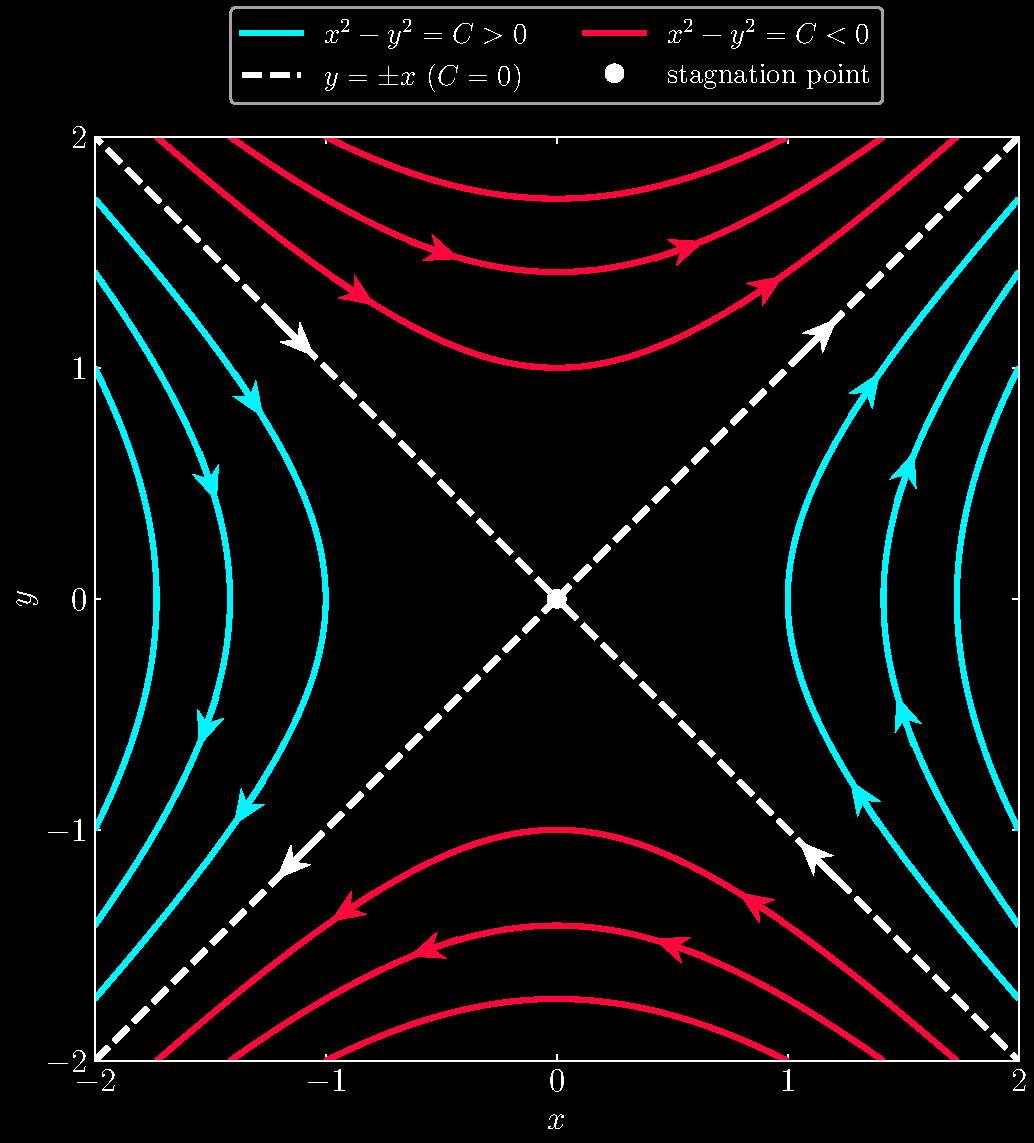
\includegraphics[width=0.9\textwidth]{../chap3-code/chap3ex3.6a.pdf}
	\end{center}
	\item Define \( \pmb{u} = \!\left( Sy, Sx \right) \). From the definition of the (symmetric) strain rate tensor
	\[
		S_{ij} = \frac{1}{2}\!\left( \frac{\partial u_{i}}{\partial x_{j}} + \frac{\partial u_{j}}{\partial x_{i}} \right)
	\]
	from which we compute
	\[
		S_{ij} = \begin{bmatrix}
			\frac{\partial u}{\partial x} & \frac{1}{2}\!\left( \frac{\partial v}{\partial x} + \frac{\partial u}{\partial y} \right) \\
			\frac{1}{2}\!\left( \frac{\partial u}{\partial y} + \frac{\partial v}{\partial x} \right) & \frac{\partial v}{\partial y}
		\end{bmatrix}
		=
		\begin{bmatrix}
			0 & S \\
			S & 0
		\end{bmatrix}
	\]
	\item From the definition of the (antisymmetric) rotation tensor
	\[
		R_{ij} = \frac{\partial u_{i}}{\partial x_{j}} - \frac{\partial u_{j}}{\partial x_{i}} 
	\]
	from which we compute
	\[
		R_{ij} = \begin{bmatrix}
			0 & \frac{\partial u}{\partial y} - \frac{\partial v}{\partial x} \\
			\frac{\partial v}{\partial x} - \frac{\partial u}{\partial y} & 0
		\end{bmatrix} 
		=
		\begin{bmatrix}
			0 & 0 \\
			0 & 0
		\end{bmatrix}
	\]
	\item From the strain rate tensor, compute the determinant as (and set equal to zero)
	\[
		\det\!\left\lvert S_{ij} - \lambda \delta_{ij} \right\rvert = \det\!\left\lvert \begin{bmatrix}
			-\lambda & S \\
			S & -\lambda
		\end{bmatrix} \right\rvert
		= \lambda^{2} - S^{2} = 0
	\]
	which has solutions \( \lambda^{\!\left( 1 \right)} = S \) and \( \lambda^{\!\left( 2 \right)} = -S \). The corresponding normalized eigenvector solutions are
	\[
		\pmb{b}^{\!\left( 1 \right)} = \begin{bmatrix}
			1 / \sqrt{2} \\
			1 / \sqrt{2}
		\end{bmatrix}, \quad
		\pmb{b}^{\!\left( 2 \right)} = \begin{bmatrix}
			-1 / \sqrt{2} \\
			1 / \sqrt{2}
		\end{bmatrix}
	\]
	Using the eigenvectors, assemble the transformation matrix
	\[
		\pmb{C} = \begin{bmatrix}
			\pmb{b}^{\!\left( 1 \right)} & \pmb{b}^{\!\left( 2 \right)}
		\end{bmatrix}
		=
		\begin{bmatrix}
			1 / \sqrt{2} & -1 / \sqrt{2} \\
			1 / \sqrt{2} & 1 / \sqrt{2}
		\end{bmatrix}
	\]
	which corresponds to a 45-degree rotation of the axes. Lastly, derive the transformed strain rate tensor \( \pmb{S} \) in the rotated frame as 
	\[
		\pmb{C}^{\textsc{T}}\pmb{S}\pmb{C} = \pmb{S}' = \begin{bmatrix}
			S & 0 \\
			0 & -S
		\end{bmatrix} 
	\]
	\item Akin to Example 3.5, the flow lines are hyperbolae, albeit asymptotically bounded by the diagonals rather than by the axes. When oriented around the principal axes and \( S > 0 \), fluid elements expand in the \( x' \)-direction and contract in the \( y' \)-direction.
\end{enumerate}

% QUESTION 7
\qs{3.7}{At the instant shown in Figure 3.2b, the \( \!\left( u,v \right) \)-velocity field in Cartesian coordinates is \( u = A \!\left( y^{2} - x^{2} \right) / \!\left( x^{2} + y^{2} \right)^{2} \), and \( v = -2Axy / \!\left( x^{2} + y^{2} \right)^{2} \) where \( A \) is a positive constant. Determine the equations for the streamlines by rearranging the first equality in (3.7) to read \( udy - vdx = 0 = \!\left( \partial \psi / \partial y \right)dy + \!\left( \partial \psi / \partial x \right)dx \) and then looking for a solution in the form \( \psi \!\left( x,y \right) =  \) const.}

Taking the tangency requirement \( dx / u = dy / v \), multiply by \( uv \) and bring the terms to one side to derive
\[
	udy - vdx = 0 
\]
By the method of exact equations, we can identify a candidate for \( \psi \) if and only if \( \partial M / \partial y = \partial N / \partial x \) for \( M = -v \) and \( N = u \). Compute
\begin{align*}
	\frac{\partial }{\partial y}\!\left[ \frac{2Axy}{\!\left( x^{2} + y^{2} \right)^{2}} \right] & = \frac{2Ax}{\!\left( x^{2} + y^{2} \right)^{2}} - \frac{8Axy^{2}}{\!\left( x^{2} + y^{2} \right)^{3}} \\
	 & = \frac{2A \!\left( x^{3} - 3xy^{2} \right)}{\!\left( x^{2} + y^{2} \right)^{3}} \\ 
	\frac{\partial }{\partial x}\!\left[ \frac{A \!\left( y^{2} - x^{2} \right)}{\!\left( x^{2} + y^{2} \right)^{2}} \right] & = -\frac{2Ax}{\!\left( x^{2} + y^{2} \right)^{2}} - \frac{4Ax \!\left( y^{2} - x^{2} \right)}{\!\left( x^{2} + y^{2} \right)^{3}} \\
																 & = \frac{2A \!\left( x^{3} - 3xy^{2} \right)}{\!\left( x^{2} + y^{2} \right)^{3}}
\end{align*}
which matches, ascertaining the existence of \( \psi \). Integrate \( -v \) with respect to \( x \) and find (by letting \( w = x^{2} + y^{2} \) and \( dw = 2x \, dx \))
\begin{align*}
	\psi \!\left( x,y \right) & = \int \frac{2Axy}{\!\left( x^{2} + y^{2} \right)^{2}} \, dx \\
				  & = Ay \int \frac{dw}{w^{2}} \\
				  & = -\frac{Ay}{x^{2} + y^{2}} + g \!\left( y \right)
\end{align*}
Differentiate with respect to \( y \) to derive
\begin{align*}
	\frac{\partial \psi}{\partial y} & = -\frac{A}{x^{2} + y^{2}} + \frac{2Ay^{2}}{\!\left( x^{2} + y^{2} \right)^{2}} + g'\!\left( y \right) \\
					 & = \frac{A \!\left( y^{2} - x^{2} \right)}{\!\left( x^{2} + y^{2} \right)^{2}} + g'\!\left( y \right) \\
					 & = \frac{A \!\left( y^{2} - x^{2} \right)}{\!\left( x^{2} + y^{2} \right)^{2}} = u
\end{align*}
forcing \( g'\!\left( y \right) = 0 \) and thus \( g \!\left( y \right) = C \) for any constant \( C \). Fix \( \psi \!\left( x,y \right) = \psi_{0} \). Then 
\[
	\psi_{0} = C - \frac{Ay}{x^{2} + y^{2}} 
\]
Multiplying through by \( x^{2} + y^{2} \) and rearranging, derive
\[
	x^{2} + \!\left( y + \frac{\beta}{2} \right)^{2} = \!\left( \frac{\beta}{2} \right)^{2}, \quad x \neq 0 
\]
where \( \beta = A / \!\left( \psi_{0} - C \right) \). The streamlines are then circles with center \( \!\left( 0, -\beta / 2 \right) \) and radius \( \abs{\beta} / 2 \). One final step: we have an edge case where \( \psi_{0} = C \), rendering \( \beta \) undefined. Then we find
\[
	-\frac{Ay}{x^{2} + y^{2}} = 0 \quad \implies \quad y = 0, \quad x \neq 0
\]
Note that due to the \( x^{2} + y^{2} \) term in the denominator, the streamlines and the velocities are undefined at the origin \( \!\left( 0,0 \right) \).

\vspace{12pt}

% QUESTION 10
\qs{3.10}{Compute and compare the streamline, path line, and streak line that pass through \( \!\left( 1,1,0 \right) \) at \( t = 0 \) for the following Cartesian velocity field \( \pmb{u} = \!\left( x,-yt,0 \right) \).}

\textbf{Streamline}.
By equation (3.7), derive
\[
	\frac{d y}{d x} = \frac{v}{u} = -\frac{yt}{x} 
\]
which, after separating variables and integrating, resolves to
\[
	 y = Cx^{-t}
\]
Since \( w = 0 \), there is no variation in \( z \), leaving only one equation in \( \!\left( x,y \right) \). At \( t = 0 \), we have \( y = C \), requiring \( C = 1 \). The streamline equation is \( y = 1 \), \( z = 0 \) for \( x > 0 \); recall from our derivation of \( dy/dx \) that \( x \) is in the denominator, and the streamline cannot be defined at \( x = 0 \). Physically, at \( t = 0 \) and \( x = 0 \), the velocity is \( \pmb{u} = \!\left( 0,0,0 \right) \), for which no streamlines can exist.

\textbf{Path-line}. Define \( \pmb{r} = \!\left[ x \!\left( t \right),y \!\left( t \right) \right] \) and set 
\[
	\frac{d x}{d t} = u = x, \quad \frac{d y}{d t} = v = -yt, \quad \frac{d z}{d t} = w = 0
\]
Separate variables and integrate to show
\[
	x \!\left( t \right) = x_{0}e^{t}, \quad y \!\left( t \right) = y_{0}e^{-t^{2}/2}, \quad z \!\left( t \right) = z_{0}
\]
By the path-line trajectory intercept requirement, \( x \!\left( 0 \right) = x_{0} = 1 \), \( y \!\left( 0 \right) = y_{0} = 1 \), and \( z \!\left( 0 \right) = z_{0} = 0 \). The path-line component equations are 
\begin{align*}
	x \!\left( t \right) & = e^{t} \\
	y \!\left( t \right) & = e^{-t^{2}/2} \\ 
	z \!\left( t \right) & = 0
\end{align*}
To do away with the \( t \) term, write \( t = \ln\!\left(x\right) \) and substitute into \( y \!\left( t \right) \):
\[
	y \!\left( x \right) = e^{-\!\left[ \ln\!\left(x\right) \right]^{2} / 2} = x^{-\ln\!\left(x\right)/2}, \quad z = 0, \quad x > 0
\]
where once again we must have \( x > 0 \) as \( x \!\left( t \right) = e^{t} \). Note that at \( t = 0 \) and \( \!\left( 1,1,0 \right) \), \( \!\left( dx/dt,dy/dt,dz/dt \right)= \!\left( 1,0,0 \right) \). The velocity is a horizontal vector at that point. As it turns out, the derivative of our path-line at that point is
\[
	\left.\frac{d y}{d x}\right\rvert_{x=1} = -e^{-\!\left[ \ln\!\left(x\right) \right]^{2}/2}\!\left[ \frac{\ln\!\left(x\right)}{x} \right] = 0
\]
which agrees with the direction of our velocity vector. Since the streamline must be tangent to the flow velocity, our result also comports with our streamline equation \( y = 1 \).

\textbf{Streak-line}. Consider time \( t_{0} \) which may transpire at any timestep before or after \( t \). Using our equations for \( x \), \( y \), and \( z \) for the path-line derivation, we rederive new constants for the fluid particle at \( \!\left( 1,1,0 \right) \) at that earlier time:
\begin{alignat*}{2}
	x \!\left( t_{0} \right) & = x_{0}e^{t_{0}} = 1 && \implies x_{0} = e^{-t_{0}} \\
	y \!\left( t_{0} \right) & = y_{0}e^{-t_{0}^{2}/2} = 1 && \implies y_{0} = e^{t_{0}^{2}/2} \\ 
	z \!\left( t_{0} \right) & = 0 && \implies z_{0} = 0
\end{alignat*}
Then substituting back into our component equations, find
\begin{align*}
	x \!\left( t \right) & = e^{t - t_{0}} \\
	y \!\left( t \right) & = e^{\!\left( -t^{2} + t^{2}_{0} \right)/2} \\ 
	z \!\left( t \right) & = 0
\end{align*}
This time, eliminate \( t_{0} \) by writing \( t_{0} = t - \ln\!\left(x\right) \) and substitute
\[
	y \!\left( x \right) = e^{-t \ln\!\left(x\right) + \!\left[ \ln\!\left(x\right) \right]^{2}/2} = x^{-t + \ln\!\left(x\right)/2}
\]
And finally, evaluate at \( t = 0 \) to conclude
\[
	y \!\left( x \right) = x^{\ln\!\left(x\right)/2}, \quad z = 0, \quad x > 0
\]
We summarize the results in the table below.

\begin{center}
	\renewcommand{\arraystretch}{1.8}
	\setlength{\arraycolsep}{10pt}
	\begin{tabular}{|c||c|c|}
		\hline
		\rule[-1.2em]{0pt}{3em}
		Equation & \( y \!\left( x \right) (z = 0) \) & \( x \)-domain \\
		\hline\hline
		\rule[-1.2em]{0pt}{3em}
				Streamline & \( 1 \) & \( x > 0 \) \\
		\hline
		\rule[-1.2em]{0pt}{3em}
				Path-line & \( x^{-\ln\!\left(x\right)/2} \) & \( x > 0 \) \\
		\hline
		\rule[-1.2em]{0pt}{3em}
				Streak-line & \( x^{\ln\!\left(x\right)/2} \) & \( x > 0 \) \\
		\hline
	\end{tabular}
\end{center}
\end{document}
